\documentclass{article}
\usepackage{graphicx}
\usepackage[margin=1in]{geometry}
\usepackage{dingbat}
\usepackage{placeins}
\usepackage{ragged2e}


\graphicspath{ {Images/} }

\usepackage{hyperref}
\hypersetup{
    colorlinks=true,
    linkcolor=blue,
    filecolor=magenta,      
    urlcolor=blue,
    pdftitle={Sharelatex Example},
    bookmarks=true,
    pdfpagemode=FullScreen,
}


\title{Summary of  "A Practical Attack to De-Anonymize Social Network Users"}
\author{Saranya Radhakrishnan}
\date{02/08/2015}

\begin{document}
\maketitle
\justify

Social networks have provisioned the feature of creating  groups of users with an idea of  connecting users with similar interests . The amount of private and sensitive information stored in social networking sites is greater compared to other sites , thus making the social networking sites vulnerable to attacks. The most common way of attacking these sites to steal personal information is by garnering user information from group memberships which uniquely identifies the user. 

\begin{center}
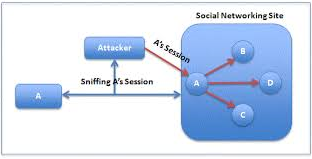
\includegraphics{AttackInGraphicalFormat}
\end{center}


The authors of the paper , "A Practical Attack to De-Anonymize Social Network Users"  have leveraged on stealing group membership of users from well known web browser history stealing attacks. This implies that whenever a user visits a malicious website,it would initiate the de-anonymization attack and pick up visitors’ identity.


The authors have further detailed their attacks based primarily on stealing history as of two types namely
 Basic attack - steals user information
 Improved attack - relies on groups instead of individual users


The paper further explains crawling experiments that were used to fetch the information about 
groups based on experiments performed on three social networks Xing, Facebook and LinkedIn. The findings of the experiment are elaborated below.

\begin{enumerate}

\item  Xing: 
The authors have demonstrated the feasibility of attacks on users of Xing social network successfully. Attacking  Xing , a moderate sized social networking medium , with approximately 8 million users (at the time of writing this paper) , resulted in extensive collection of data of the groups as well as the users of Xing. The analysis of the attack led to the findings that attacker checked 6,277 groups , implying it needed to check only 6,277 urls only instead of 8 million urls.

\item Facebook:

 Due to the enormity of facebook data the authors  decided to use a commercial crawling service to download requite user information .They extracted the group IDs and then supplied that as input to their own custom crawler to extract information about group members. The findings were as follows
The authors crawled more than  43.2 million group members from 31,853 groups in a span of 23 days using only two machines. 
\\

\item LinkedIn: 

The authors applied a  two-phase crawling method , In the first pass .they  generated 3 million hyperlinks for the observed group ID space, and then these links were supplied as input to a commercial crawling service. The authors had to perform another  crawling pass to extract information such as  group size and group description.

\end{enumerate}

After a studying other social networking sites, the authors tabulated their findings as shown below

\FloatBarrier
\begin{table}[h!]
\centering
\begin{center}
\begin{tabular}{ |p{3cm}||p{2.5cm}|p{2.5cm}|p{2.5cm}|p{2.5cm}| }
\hline
     &  Facebook& LinkedIn & Xing & MySpace  \\ 
\hline
Uses dynamic links &  \checkmark & \checkmark & \checkmark  & \checkmark  \\ 
\hline
Group Directory &  FULL & SEARCHABLE & SEARCHABLE & SEARCHABLE  \\ 
\hline
Member Directory &  FULL & FULL & SEARCHABLE  & SEARCHABLE  \\ 
\hline
Group member enumeration &  less than or equals 6,000 & less than or equals 500 & UNLIMITED & UNLIMITED  \\ 
\hline
Public member profiles &  \checkmark & \checkmark & \checkmark & \checkmark  \\ 
\hline
Vulnerable &  \checkmark & \checkmark & \checkmark & \checkmark  \\ 
\hline

\end{tabular}
\caption{VULNERABILITY COMPARISON OF SOCIAL NETWORKS}
\label{table:1}
\end{center}
\end{table}




Further the authors proposed mitigation techniques to counter the attacks as stated below
\begin{enumerate}
\item  Server­ side mitigation technique
\begin{itemize}
\item Usage of dynamic hyperlinks that would contain HTTP GET parameters with randomized tokens
\item Pass parameters through HTTP POST instead of HTTP GET in order to prevent creation of browser history.
\end{itemize}
   
\item  Client ­side mitigation technique 
\begin{itemize}
\item	Prohibit the browsers from disclosing private information through CSS by restricting the access of client-side scripts. 
\item	The users can prevent information leakage by deleting browser history periodically. 
\end{itemize}
\end{enumerate}

 
\section*{References}

\begin{enumerate}
\item  \href{http://www.cs.wustl.edu/~jain/cse571-11/ftp/social/index.html}{Image of Attack}
\end{enumerate}


Link to the repository:  \href{https://github.com/rsaranya/SecurityAlgorithm.git}{GitHub Repository}
\end{document}